\section{Proposed Method}

\begin{frame}{Proposed method}

\begin{algorithm}[H]
\caption{Training Protocol \footnote{\href{http://papers.nips.cc/paper/8025-reward-learning-from-human-preferences-and-demonstrations-in-atari}{Reward learning from human preferences anddemonstrations in Atari, \textit{Ibarz et all.}}}}

\begin{algorithmic}[1]
\STATE Run the policy in the environment and store "initial trajectories".
\STATE The annotator annotated all the "initial clips" and create the annotation buffer.
\STATE Pretrain the reward model from the annotation buffer.
\FOR{\textit{M} epochs} 
\STATE Train the policy in the environment for \textit{N} episodes with rewards from the reward model.
\STATE Sample pairs of clips from the resulting trajectories.
\STATE The annotator labels the selected pairs and puts them in the annotation buffer.
\STATE Train the reward model for \textit{K} batches from the annotation buffer.
\ENDFOR 
\end{algorithmic}
\end{algorithm}

\end{frame}

\begin{frame}
\frametitle{Policy}

\begin{itemize}
    %\item The policy receive an observation \textit{$o_t$} and it takes an action \textit{$a_t$}
    \item The reward is not taken from the environment but from a reward model
    \item The policy receives the current agent state as input and probabilities of actions as output
        
\end{itemize}

\centering
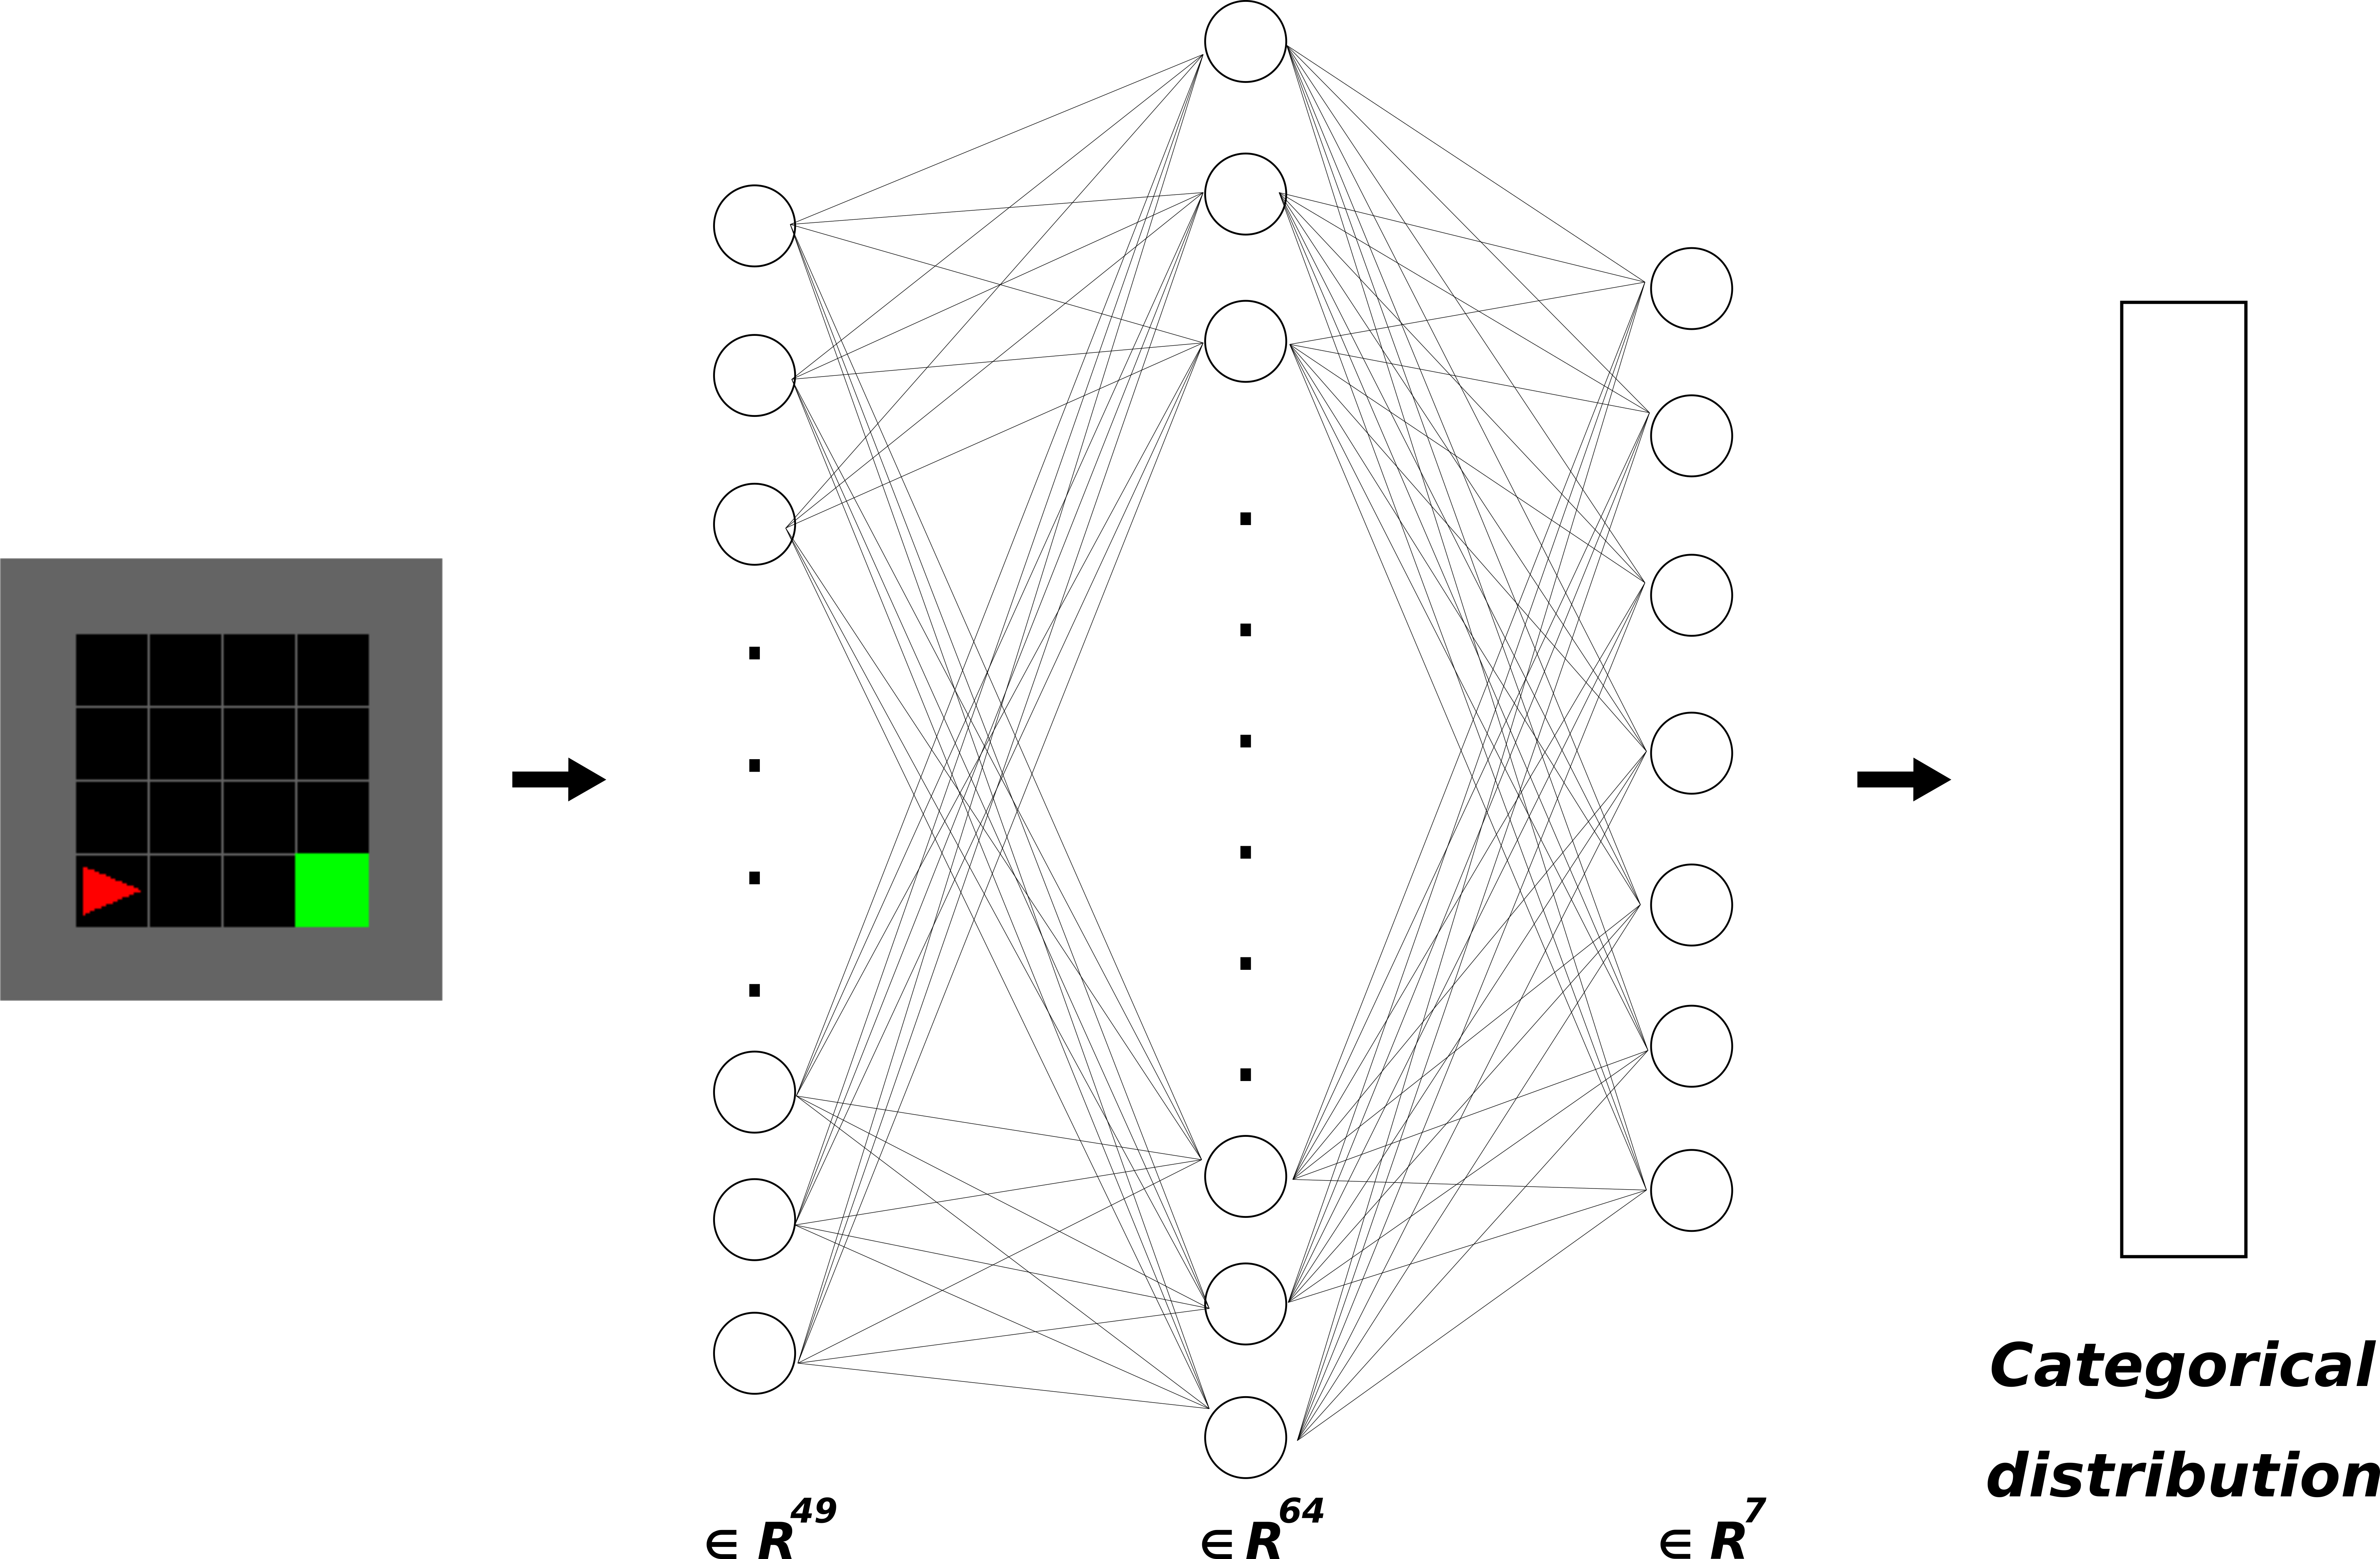
\includegraphics[width=0.6\linewidth]{images/policy.png}

\end{frame}

\begin{frame}
\frametitle{Annotator}
		\begin{itemize}
		\item The annotator gives preference feedback about pairs of clips
		\vspace{0.2cm}
		\begin{itemize}
			\item (0,1) (1,0) preferred clips
			\item (0.5,0.5) indifferent labels
			\item (0,0) discarded clips
		\end{itemize}
		
	\vspace{0.3cm}
	
		\item<2-> Human annotator vs Artificial annotator (\textit{Oracle})
		
	\end{itemize}
	\begin{columns}<2->
		\begin{column}{0.5\textwidth}
			\centering
			\footnotesize{
			\begin{tabular}{|c|c|c|c|}
				\hline
				1 & 0    & 0    & 0     \\ \hline
				1 & 0.5  & 0.25 & 0.125 \\ \hline
				1 & 0.25 & 0.5  & 0.125 \\ \hline
				1 & 1    & 1    & 10    \\ \hline
			\end{tabular}
		}
		\end{column}
		
		\begin{column}{0.5\textwidth}
			\centering
			\footnotesize{
			\begin{tabular}{|c|c|c|c|}
				\hline
				1 & 0 & 0 & 0  \\ \hline
				1 & 0 & 0 & 0  \\ \hline
				1 & 0 & 0 & 0  \\ \hline
				1 & 1 & 1 & 10 \\ \hline
			\end{tabular}
		}
		\end{column}
	\end{columns}
	
	\vspace{0.3cm}
	
	\begin{itemize}
		\item<3-> All the preferences are stored in the Annotation Buffer
	\end{itemize}
	
\end{frame}

\begin{frame}
\frametitle{Reward Model}
\begin{itemize}
    \item The Reward Model has to emulate the annotator labels
    \item It is trained to minimize the cross-entropy loss between predictions and labels
\end{itemize}

\vspace{0.2cm}

\begin{equation*}
    loss(\hat{r}) = - \sum_{(\sigma^1,\sigma^2,\mu)\in A} \mu(1)log(\hat{P}[\sigma^1 \succ \sigma^2]) + \mu(2)log(\hat{P}[\sigma^2 \succ \sigma^1])
\end{equation*}

%\vspace{0.3cm}
\begin{itemize}
    \item where
\end{itemize}

\begin{equation*}
    \hat{P}[\sigma^1 \succ \sigma^2] = \frac{exp(\sum_{o \in \sigma^1} \hat{r}(o))}{exp(\sum_{o \in \sigma^1} \hat{r}(o) + \sum_{o \in \sigma^2} \hat{r}(o))}
\end{equation*}



\end{frame}


\begin{frame}
\frametitle{Reward Model}
\begin{itemize}
    \item The Reward Model predicts a list of rewards from a clip
\end{itemize}
\vspace{0.3cm}
\centering
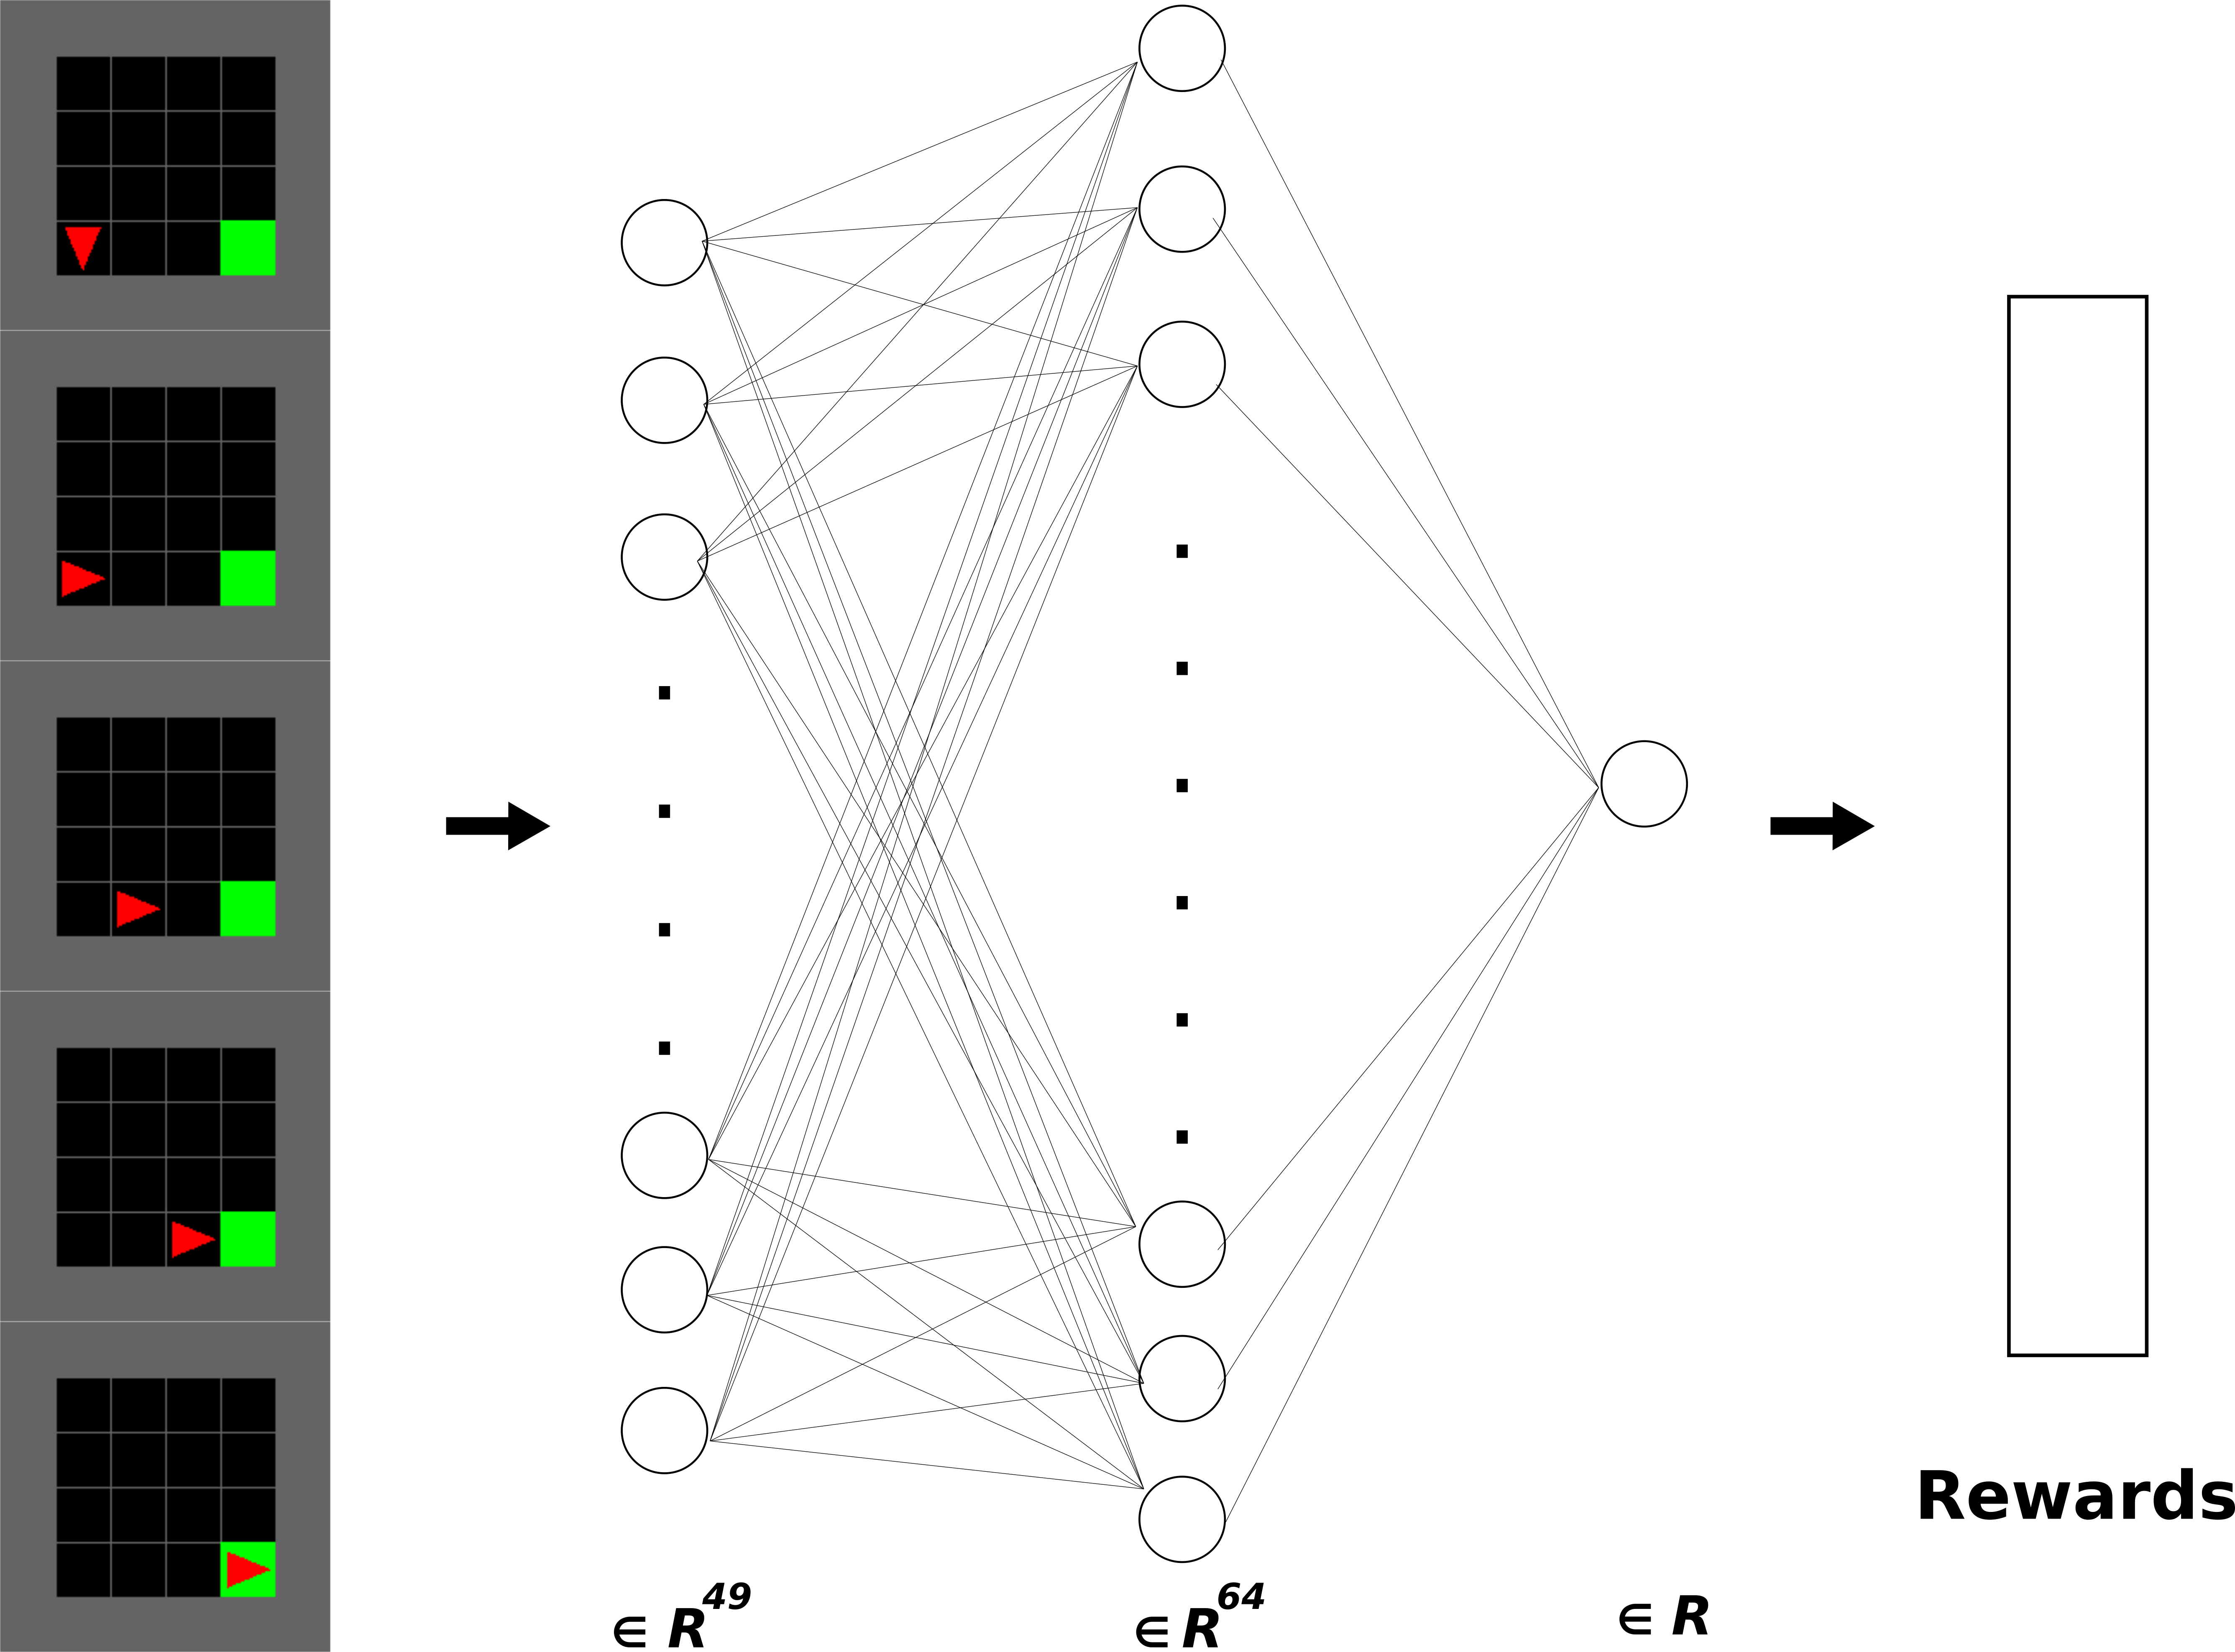
\includegraphics[width=0.55\linewidth]{images/reward.png}
\end{frame}


\begin{comment}
\subsection{IRL Components}

\begin{frame}
\frametitle{Policy}
dasdsa
\end{frame}

\begin{frame}
\frametitle{Annotator}
dasdsa
\end{frame}

\begin{frame}
\frametitle{Reward model}
\begin{itemize}
    \item bello
    \item raga
\end{itemize}
\end{frame}

\end{comment}


